\subsection{Speedup}
\textbf{Speedup} is a number that measures the relative performance of two systems processing the same problem.
More technically, it is the improvement in speed of execution of a task executed on two similar architectures with different resources \cite{wiki:Speedup}. 
Speedup can also be used as a measure of the relative speed of a parallel algorithm compared to its sequential counterpart.
The concept of speedup is connected to the Amdahl's law.
The curve of the speedup depends on the number of processors P, the size N of the problem, and the time complexity of an algorithm.
So in most cases, speedup functions, plotted considering the same algorithm launched on a different number of processors, are not linear but present a particular trend that can be explained in the light of machine characteristics, algorithm complexity, parallelizable portions, framework used, etc.

\subsection{Efficiency}
Furthermore, it exists another metric that measure the quality of a parallel algorithm, the \textbf{efficiency}. It measures how many times a parallel version of an algorithm executed on P processors is faster than the same parallel version executed on only one processor.
In particular, the relative efficiency is:
\begin{equation}
    E_r=\frac{T_1}{P*T_P} 
\end{equation}
where $T_1$ is the time required to execute the algorithm on one processor, $P$ is the number of processors and $T_P$ is the time required to execute the same algorithm on $P$ processors.
% Non so se inserire o meno la formula dello speedup relativo

\subsection{Amdahl's law}
\textbf{Amdahl's law} is a formula which gives the theoretical speedup of an algorithm when only a percentage $p$ of the algorithm can be parallelized.
Amdahl's law is often used in parallel computing to predict the theoretical speedup when using multiple processors.
For example, if a program needs 20 hours to complete using a single thread, but a one-hour portion of the program cannot be parallelized, therefore only the remaining 19 hours' (p = 0.95) execution time can be parallelized,
then regardless of how many threads are devoted to a parallelized execution of this program, the minimum execution time cannot be less than one hour.
Hence, the theoretical speedup is limited to at most 20 times the single thread performance, $(\frac{1}{1-p}=20)$.

Amdahl's law can be formulated in the following way:
\begin{equation}
    S_{latency}(s)=\frac{1}{(1-p)+\frac{p}{s}} 
\end{equation}

where:
\begin{itemize}
    \item $S_{latency}$ is the theoretical speedup of the execution of the whole task;
    \item $s$ is the speedup of the part of the task that benefits from improved system resources;
    \item $p$ is the proportion of execution time that the part benefiting from improved resources originally occupied.
\end{itemize}

Furthermore, these equations
\begin{equation}
    \left\{
        \begin{aligned}
            &S_{latency}(s)\leq \frac{1}{(1-p)}  \\
            &\lim_{s \to \infty} S_{latency}(s)= \frac{1}{(1-p)+\frac{p}{s}} \\
        \end{aligned}
    \right.
\end{equation}
show that the theoretical speedup of the execution of the whole task increases with the improvement of the resources of the system and that regardless of the magnitude of the improvement, the theoretical speedup is always limited by the part of the task that cannot benefit from the improvement.

Amdahl's law can be used to compute the upper bound of the speedup of an algorithm, assuming that the speedup of the parallel part is equal to the number of processes.
% può essere usata per calcolare un upper bound allo speedup supponendo che lo speedup della parte parallela sia pari al numero di processi

\subsection{An analytical approach for calculating the speedup upper bound}
As said before, in order to use Amdahl's law to calculate an upper bound for the speedup of a parallel program, we need to estimate the percentage $p$ of execution time of the part that could benefit from parallelization in the sequential program.
\\A possible approach for estimating $p$ is to manually calculate the costs of the parallelizable and sequential parts of the algorithm by counting the number of elemental operations performed. The implicit hypotesis is that each elemental operation approximately takes the same time, thus the execution time of an algorithm would be proportional to it's cost. Notice how using the asymptotic complexity would lead to a wrong estimation, because it ignores lower order terms and multiplication factors that could be significant for determining the program execution time.
\\In this paragraph we will see an example application of this approach for estimating $p$ for our version of Tarjan's algorithm parallelized with CUDA. For further information on this algorithm, see \ref{alg:cuda_only}.

\noindent The functions called by the sequential algorithm are \verb|cuda_graph_load_from_file()| \verb|scc_set_init()| \verb|preprocess()| \verb|cuda_graph_to_graph()| \verb|graph_tarjan_foreach()| \verb|graph_num_vertex()| \verb|scc_set_save_to_file()| \verb|graph_free()| \verb|cuda_graph_free()| \verb|scc_set_free()| and \verb|free()|. From the taken measurements, we determined that most of the functions' execution time is negligible. The ones that influence the execution time the most are \verb|cuda_graph_load_from_file()| \verb|preprocess()| \verb|cuda_graph_to_graph()| and \verb|graph_tarjan_foreach()|. For each of these functions we calculate the cost function $T(\cdot)$, with:
\begin{itemize}
  \item $v$: number of vertices
  \item $e$: number of edges
  \item $v_1$: vertices not deleted after preprocess
  \item $v_2$: vertices deleted after preprocess
  \item $e_1$: edges not deleted during preprocess.
\end{itemize}

\noindent The function \verb|cuda_graph_load_from_file()| is used to read the graph from a binary file in a format that is compatible with CUDA elaborations. The cost of this function depends on the number of vertices and edges in the graph: $T_1(v,e)=9v+4e+11$.
\\ The function \verb|preprocess()| is used to delete trivial SCCs from the graph. This is the only function that will be parallelized by CUDA. The cost of this function depends on the number of vertices and edges in the graph: $T_2(v,e)=3ve+13v+6$
\\ The function \verb|cuda_graph_to_graph()| is used to convert the CUDA-friendly representation of the graph into an adjacency map representation used by Tarjan's algorithm. The cost of this function depends on the number of vertices and edges in the graph after the preprocessing, as well as the number of deleted vertices: $T_3(v_1,v_2,e_1)=10v_1+24e_1+3v_2+6$
\\ The function \verb|graph_tarjan_foreach()| actually executes Tarjan's algorithm on the preprocessed graph. Calculating the cost of this function is not trivial, for it strongly depends on the topology of the input graph. Factors that influence the cost of this function are: number of connected components, number of SCCs, degree of each vertex in the graph. In order to calculate the cost, here we assume to execute the function on a fully connected graph: $T_4(v,e)=12v^2+58v+38$.

\noindent Given the assumption made for estimating the cost of \verb|graph_tarjan_foreach()|, we have that $e=v(v-1)$, $v_1=v$, $e_1=e$ and $v_2=0$. Thus
\begin{align*}
  p(v) & =\frac{T_2(v,e)}{T_1(v,e)+T_2(v,e)+T_3(v_1,v_2,e_1)+T_4(v,e)} \\
       & =\frac{3ve+13v+6}{12v^2+80v+4e+3ve+10v_1+24e_1+3v_2+61} \\
       & =\frac{3v^3-3v^2+13v+6}{3v^3+37v^2+62v+61}
\end{align*}
For instance, with a fully connected graph with $100$ vertices, the fraction of parallelizable time is $p(100)=0.88$. By applying Amdahl's law the maximum theoretical speedup is:
\begin{align*}
  S_{max}(P)=\frac{1}{0.12+\frac{0.88}{P}}=\frac{P}{0.12P+0.88}
\end{align*}
\begin{center}
  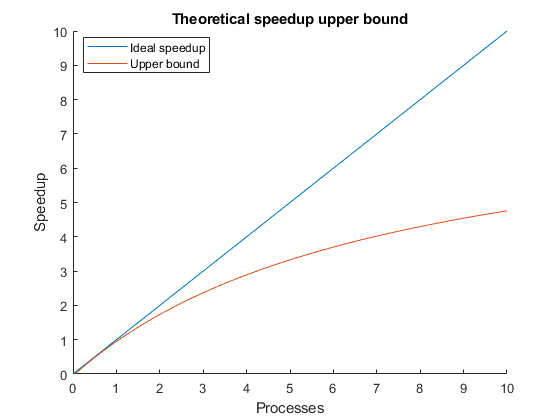
\includegraphics[scale=1]{img/untitled.png}
\end{center}

\subsection{Our methodology for calculating the speedup upper bound}
\noindent The analytical approach seen before has the following problems:
\begin{itemize}
  \item Manually calculating the cost of the algorithm is time-consuming
  \item The correctness of the result relies on the strong hypothesis that execution time will be proportional to the cost of the algorithm
  \item The cost of the algorithm (and thus $p$) strongly depends on the input size of the algorithm
  \item Different algorithm will have different parallelized sections (for example with CUDA we parallelize the preprocessing of the graph, while with MPI we parallelized Tarjan's algorithm)
\end{itemize}
For these reasons in the following measurements we applied Amdahl's law by calculating $p$ directly from the measurements of the corresponding sequential algorithm executed with the right input. For instance, in order to plot the speedup upper bound for the CUDA algorithm described in \ref{alg:cuda_only}, we measure $t_{preprocess}$ (the time needed by the sequential program to pre-process the graph) and $t_{elapsed}$ (total running time of the sequential algorithm), such that we calculate
\begin{align*}
  p = \frac{t_{preprocess}}{t_{elapsed}}
\end{align*}
for each input graph. After that we calculate the maximum theoretical speedup by applying Amdahl's law as seen before. In the following chapters all of the upper bounds have been determined with this approach.

\subsection{Input graphs used for the measurements}
The implemented algorithms have been tested with different graphs, to test them under difference circumstances and to have a reliable estimate of the performances.
Specifically, the following it is tested:
\begin{itemize}

    \item Fully connected graph;
      \\A fully connected graph with 12500 nodes (each node is connected via edges to all other nodes in the graph).
      \\Such a graph was created using the sgg tool, in the root directory \textit{./tarjan/} is as follows: 
      \\\textit{./bin/sgg.out ./data/fully-connected-12500.bin 12500 0}

    \item Fully disconnected graph;
    \\A fully disconnected graph with 1000000 nodes and each node has no edge.
    \\Such a graph was created using the sgg tool, in the root directory \textit{./tarjan/} is as follows: 
    \\\textit{./bin/sgg.out ./data/fully-disconnected-1000000.bin 1000000 1}

    \item Random graph;
    \\Randomly generated graphs with variable number of nodes. The number of outgoing edges of each node is distributed according to the Bernoulli distribution with a given mean and variance. The Bernoulli distribution was used since it can be seen as a Gaussian distribution that operates only with positive values. 
    \\Such a graph was created using the rsg tool, in the root directory \textit{./tarjan/} is as follows: 
    \\\textit{./bin/rsg.out ./data/random-150000.bin 150000 1 0.5}
    \\\textit{./bin/rsg.out ./data/random-250000.bin 250000 1 0.5}
    \\\textit{./bin/rsg.out ./data/random-500000.bin 500000 1 0.5}
    \\In generating the graphs, a low mean was chosen to avoid creating graphs in which there is only one SSC that includes all nodes in the graph.
    \begin{itemize}
      \item random with 150000 nodes;
      \item random with 250000 nodes;
      \item random with 500000 nodes;
    \end{itemize}
    
    \item Tile graph;
    \\Graphs generated from a seed graph. Using an integer $n$, a graph with $2^n$ replications of the seed graph is generated while retaining all the edges already present in the seed. In addition, edges are added between the different seeds of the final graph according to a Bernoulli distribution.
    \\Such a graph was created using the rgg tool, in the root directory \textit{./tarjan/} is as follows: 
    \\\textit{./bin/rgg.out ./data/seed.bin ./data/tile-52000.bin 9 0.25}
    \\\textit{./bin/rgg.out ./data/seed.bin ./data/tile-205000.bin 11 0.25}
    \\\textit{./bin/rgg.out ./data/seed.bin ./data/tile-410000.bin 12 0.25}
    \\\textit{./bin/rgg.out ./data/seed.bin ./data/tile-820000.bin 13 0.25}
    \\The seed graph used was accurately chosen to avoid the formation of one single large SCC in the final graph after its replication.
    \begin{itemize}
      \item tile with 52000 nodes;
      \item tile with 205000 nodes;
      \item tile with 410000 nodes;
      \item tile with 820000 nodes;
    \end{itemize}
    
\end{itemize}